\chapter{Resultados y Discusión} \label{sec:Resultados}

\section{Pruebas Realizadas con el Sistema en Funcionamiento}

Se realizaron 4 pruebas de esfuerzos diferentes entre ellas están las sentadillas con pesas de 25Kg, la maquina prensa sin pesas, correr por 10 metros y realizar 7 saltos; las dos primeras pruebas se hicieron en el gimnasio de la Universidad Tecnológica de Bolívar como se puede observar a continuación en la figura \ref{fig:Pruebas}.

\begin{figure}[H]
 \centering
  \subfloat[Sentadillas]{
   \label{fig:Sentadillas}
    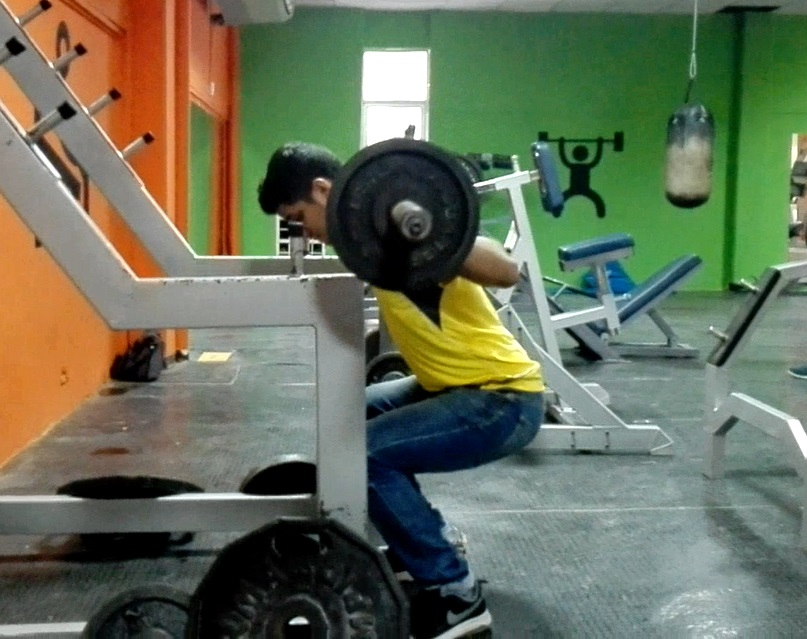
\includegraphics[width=0.244\textwidth]{./image/Sentadillas.jpg}}
    \subfloat[Prensa]{
   \label{fig:Prensa}
    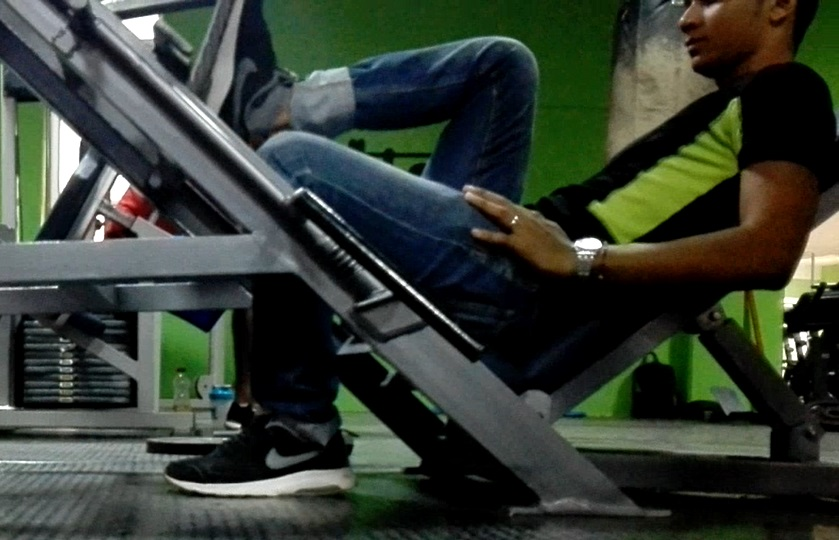
\includegraphics[width=0.3\textwidth]{./image/Prensa.jpg}}\\
    \subfloat[Correr]{
   \label{fig:Correr}
    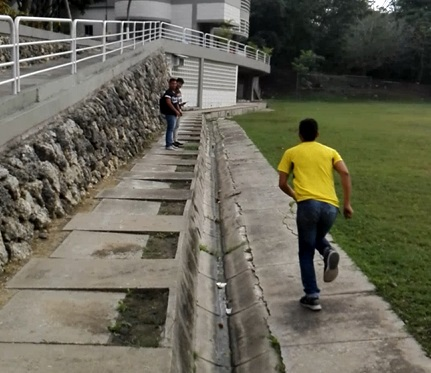
\includegraphics[width=0.3\textwidth]{./image/Correr.jpg}}
    \subfloat[Saltos]{
   \label{fig:Saltos}
    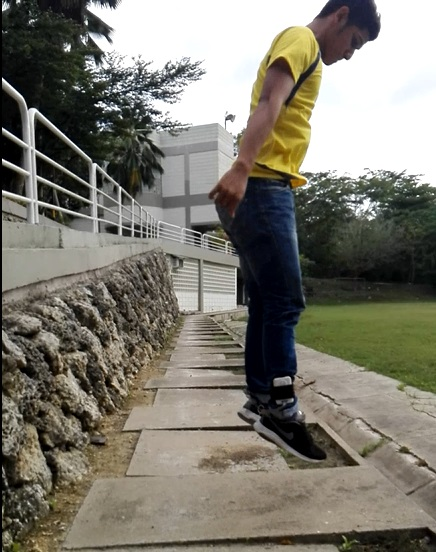
\includegraphics[width=0.205\textwidth]{./image/Saltos.jpg}}
 \caption{Pruebas realizadas.}
 \label{fig:Pruebas}
\end{figure}

\begin{table}[H]
\small
%\footnotesize
%\scriptsize
%\tiny
\begin{center}
\resizebox{10cm}{!} {
\begin{tabular}{| c | c | c | c | c | c | c | c | c | c | c | c |}
\hline
\multicolumn{6}{| c |}{\textbf{Sentadillas con 25Kg}} & \multicolumn{6}{| c |}{\textbf{Saltos}}\\
 \hline
\textbf{Sensor 1} & \textbf{Sensor 2} & \textbf{Sensor 3} & \textbf{Sensor 4} & \textbf{Sensor 5} & \textbf{Tiempo} & \textbf{Sensor 1} & \textbf{Sensor 2} & \textbf{Sensor 3} & \textbf{Sensor 4} & \textbf{Sensor 5} & \textbf{Tiempo}\\ 
 \hline
1,34 &	1,08 &	0,96 &	0,95 &	1,06 &	0,3 & 1,00 & 0,96 &	0,96 & 0,98 & 0,98 & 0,3\\
\hline
1,37 &	1,01 &	0,97 &	0,95 &	1,05 &	0,6 & 1,00 & 0,96 & 0,99 & 0,98 & 0,98 & 0,6\\
\hline
1,38 &	1,03 &	0,96 &	0,95 &	0,99 &	0,9 & 1,03 & 0,96 & 0,97 & 0,98 & 0,98 & 0,9\\
\hline
1,37 &	1,02 &	0,95 &	0,96 &	1,00 &	1,2 & 1,06 & 0,95 & 0,95 & 0,97 & 0,99 & 1,2\\
\hline
1,40 &	1,03 &	0,96 &	0,95 &	0,98 &	1,4 & 1,17 & 0,93 & 0,94 & 0,96 & 0,98 & 1,4\\
\hline
1,40 &	1,07 &	0,97 &	0,95 &	0,97 &	1,7 & 1,13 & 0,97 & 1,01 & 0,96 & 1,01 & 1,7\\
\hline
1,30 &	1,10 &	0,96 &	0,95 &	0,98 &	2,0 & 1,30 & 0,94 & 0,95 & 0,94 & 1,26 & 2,0\\
\hline
1,41 &	1,08 &	0,96 &	0,95 &	0,98 &	2,3 & 1,21 & 0,95 & 0,96 & 0,96 & 1,04 & 2,3\\
\hline
1,35 &	1,08 &	0,94 &	0,95 &	0,98 &	2,6 & 1,56 & 1,02 & 0,96 & 0,95 & 1,03 & 2,6\\
\hline
1,37 &	0,99 &	0,96 &	0,94 &	1,05 &	2,9 & 1,09 & 0,96 & 1,01 & 0,96 & 1,02 & 2,9\\
\hline
1,35 &	0,99 &	0,95 &	0,96 &	1,04 &	3,2 & 1,15 & 0,97 & 0,98 & 0,97 & 0,97 & 3,2\\
\hline
1,36 &	1,02 &	0,94 &	0,95 &	0,98 &	3,5 & 1,36 & 0,94 & 0,97 & 0,96 & 0,95 & 3,5\\
\hline
1,38 &	1,07 &	0,97 &	0,96 &	1,01 &	3,7 & 1,14 & 0,95 & 0,96 & 0,96 & 0,97 & 3,7\\
\hline
1,39 &	1,10 &	0,96 &	0,96 &	0,95 &	4,0 & 1,42 & 0,95 & 0,95 & 0,95 & 0,95 & 4,0\\
\hline
1,29 &	1,08 &	0,96 &	0,95 &	0,97 &	4,3 & 1,39 & 0,97 & 0,97 & 0,96 & 1,05 & 4,3\\
\hline
1,32 &	0,96 &	0,96 &	0,96 &	0,99 &	4,6 & 1,22 & 0,97 & 0,96 & 0,95 & 0,97 & 4,6\\
\hline
1,30 &	0,97 &	0,99 &	0,95 &	0,92 &	4,9 & 1,40 & 1,04 & 0,94 & 0,95 & 1,03 & 4,9\\
\hline
1,29 &	0,97 &	0,95 &	0,93 &	0,98 &	5,2 & 1,40 & 0,96 & 0,95 & 0,95 & 1,02 & 5,2\\
\hline
1,31 &	1,00 &	0,97 &	0,95 &	0,94 &	5,5 & 1,58 & 0,97 & 0,95 & 0,95 & 1,11 & 5,5\\
\hline
1,33 &	1,02 &	0,95 &	0,96 &	0,95 &	5,8 & 1,31 & 0,95 & 0,95 & 0,95 & 0,99 & 5,8\\
\hline
1,35 &	1,04 &	0,96 &	0,95 &	0,95 &	6,1 & 1,18 & 0,95 & 0,96 & 0,96 & 0,95 & 6,1\\
\hline
1,30 &	1,12 &	0,96 &	0,95 &	0,95 &	6,3 & 1,10 & 0,95 & 0,96 & 0,98 & 0,94 & 6,3\\
\hline
1,35 &	1,11 &	0,95 &	0,95 &	0,96 &	6,6 & 1,21 & 0,96 & 0,96 & 0,96 & 0,95 & 6,6\\
\hline
1,31 &	1,03 &	0,95 &	0,95 &	0,96 &	6,9 & 1,13 & 0,95 & 0,96 & 0,96 & 0,95 & 6,9\\
\hline
1,32 &	1,03 &	0,95 &	0,95 &	0,96 &	7,2 & 1,20 & 0,95 & 0,97 & 0,95 & 0,96 & 7,2\\
\hline
1,30 &	1,01 &	0,95 &	0,95 &	0,98 &	7,5 & 1,49 & 0,96 & 0,96 & 0,96 & 1,03 & 7,5\\
\hline
1,39 &	1,02 &	0,95 &	0,95 &	0,95 &	7,8 & 1,28 & 0,99 & 0,96 & 0,95 & 1,17 & 7,8\\
\hline
1,36 &	1,06 &	0,96 &	0,95 &	1,01 &	8,1 & 0,97 & 1,03 & 0,95 & 0,95 & 1,13 & 8,1\\
\hline
1,36 &	1,09 &	0,97 &	0,94 &	1,05 &	8,4 & 1,29 & 0,95 & 0,96 & 0,96 & 0,97 & 8,4\\
\hline
1,38 &	1,04 &	0,95 &	0,95 &	0,95 &	8,7 & 1,41 & 0,98 & 0,97 & 0,96 & 0,97 & 8,7\\
\hline
1,39 &	1,00 &	0,96 &	0,95 &	0,96 &	8,9 & 1,17 & 0,97 & 0,96 & 1,00 & 1,13 & 8,9\\
\hline
1,35 &	1,01 &	0,95 &	0,95 &	0,97 &	9,2 & 1,14 & 0,97 & 0,97 & 0,99 & 0,99 & 9,2\\
\hline
1,37 &	1,02 &	0,95 &	0,94 &	0,94 &	9,5 & 1,22 & 0,95 & 0,96 & 0,97 & 0,97 & 9,5\\
\hline
1,40 &	1,01 &	0,97 &	0,95 &	1,00 &	9,8 & 1,20 & 0,95 & 0,97 & 0,97 & 0,97 & 9,8\\
\hline
1,38 &	1,07 &	0,95 &	0,98 &	0,98 &	10,1 & 1,19 & 0,95 & 0,96 & 0,95 & 1,00 & 10,1\\
\hline
1,37 &	1,08 &	0,95 &	0,94 &	0,97 &	10,4 & 1,06 & 0,96 & 0,96 & 0,98 & 0,95 & 10,4\\
\hline
1,34 &	1,06 &	0,95 &	0,96 &	0,98 &	10,7 & 1,05 & 0,95 & 0,97 & 0,97 & 0,94 & 10,7\\
\hline
1,37 &	0,99 &	0,95 &	0,96 &	0,96 &	11,0 & 1,03 & 1,01 & 0,97 & 0,96 & 0,97 & 11,0\\
\hline
1,37 &	0,99 &	0,95 &	0,95 &	0,96 &	11,3 & 1,32 & 0,96 & 1,00 & 0,95 & 0,95 & 11,3\\
\hline
1,35 &	1,02 &	0,95 &	0,95 &	0,96 &	11,5 & 1,25 & 0,97 & 0,98 & 0,97 & 1,09 & 11,5\\
\hline
1,41 &	1,00 &	0,95 &	0,95 &	0,98 &	11,8 & 1,32 & 0,97 & 0,95 & 0,95 & 1,03 & 11,8\\
\hline
1,41 &	1,08 &	0,96 &	0,95 &	0,99 &	12,1 & 1,35 & 1,17 & 0,95 & 0,96 & 1,20 & 12,1\\
\hline
1,45 &	1,08 &	0,95 &	0,95 &	0,98 &	12,4 & 1,22 & 1,16 & 0,96 & 0,95 & 1,04 & 12,4\\
\hline
1,40 &	1,01 &	0,98 &	0,95 &	0,97 &	12,7 & 1,31 & 0,98 & 0,98 & 0,97 & 1,00 & 12,7\\
\hline
1,34 &	0,96 &	0,95 &	0,93 &	0,96 &	13,0 & 1,55 & 0,96 & 0,95 & 0,96 & 1,11 & 13,0\\
\hline
1,32 &	0,94 &	0,95 &	0,97 &	0,94 &	13,3 & 1,47 & 0,95 & 0,95 & 0,97 & 0,97 & 13,3\\
\hline
1,32 &	0,97 &	0,95 &	0,96 &	0,95 &	13,6 & 1,41 & 0,94 & 0,95 & 0,95 & 0,98 & 13,6\\
\hline
1,44 &	0,99 &	0,95 &	0,94 &	0,94 &	13,8 & 1,32 & 0,95 & 0,95 & 0,95 & 0,97 & 13,8\\
\hline
1,40 &	1,04 &	0,95 &	0,95 &	0,96 &	14,1 & 1,28 & 0,96 & 0,96 & 0,97 & 0,96 & 14,1\\
\hline
1,38 &	1,08 &	0,94 &	0,95 &	0,97 &	14,4 & 1,22 & 0,96 & 0,96 & 0,99 & 0,97 & 14,4\\
\hline
1,40 &	1,04 &	0,95 &	0,95 &	0,96 &	14,7 & 1,20 & 0,95 & 0,95 & 0,96 & 0,95 & 14,7\\
\hline
1,37 &	1,00 &	0,95 &	0,94 &	0,94 &	15,0 & 1,48 & 0,95 & 0,95 & 0,97 & 1,23 & 15,0\\
\hline
1,38 &	1,01 &	0,95 &	0,95 &	0,93 &	15,3 & 1,34 & 0,95 & 0,95 & 0,95 & 0,97 & 15,3\\
\hline
1,37 &	1,00 &	0,95 &	0,96 &	0,94 &	15,6 & 1,44 & 0,96 & 0,97 & 0,99 & 1,01 & 15,6\\
\hline
1,37 &	1,01 &	0,95 &	0,95 &	0,96 &	15,9 & 1,64 & 0,95 & 0,95 & 0,95 & 1,21 & 15,9\\
\hline
1,38 &	1,01 &	0,95 &	0,95 &	0,95 &	16,2 & 1,36 & 0,95 & 0,95 & 0,96 & 1,11 & 16,2\\
\hline
1,44 &	1,03 &	0,95 &	0,95 &	0,97 &	16,4 & 1,74 & 0,99 & 0,96 & 0,96 & 1,01 & 16,4\\
\hline
1,39 &	1,07 &	0,96 &	0,95 &	0,98 &	16,7 & 1,59 & 0,96 & 0,96 & 0,98 & 1,09 & 16,7\\
\hline
1,36 &	1,04 &	0,95 &	0,96 &	0,97 &	17,0 & 1,43 & 0,96 & 0,95 & 0,97 & 0,99 & 17,0\\
\hline
1,36 &	0,97 &	0,95 &	0,96 &	0,95 &	17,3 & 1,32 & 0,92 & 0,96 & 0,95 & 0,94 & 17,3\\
\hline
1,33 &	0,97 &	0,93 &	0,95 &	0,98 &	17,6 & 1,26 & 0,95 & 0,98 & 0,96 & 0,95 & 17,6\\
\hline
1,37 &	0,99 &	0,95 &	0,97 &	0,93 &	17,9 & 1,27 & 0,95 & 0,97 & 0,96 & 0,95 & 17,9\\
\hline
1,36 &	1,01 &	0,95 &	0,96 &	0,99 &	18,2 & 1,30 & 0,95 & 0,96 & 1,02 & 1,07 & 18,2\\
\hline
1,38 &	0,98 &	0,95 &	0,95 &	0,97 &	18,5 & 1,36 & 0,96 & 0,95 & 0,96 & 1,00 & 18,5\\
\hline
1,40 &	1,00 &	0,93 &	0,95 &	0,97 &	18,8 & 1,37 & 0,95 & 0,96 & 0,95 & 1,00 & 18,8\\
\hline
1,39 &	1,01 &	0,95 &	0,97 &	0,98 &	19,0 & 1,32 & 0,94 & 0,95 & 0,94 & 0,95 & 19,0\\
\hline
1,39 &	1,11 &	0,95 &	0,95 &	0,97 &	19,3 & 1,55 & 0,98 & 0,95 & 0,97 & 1,11 & 19,3\\
\hline
1,42 &	1,03 &	0,95 &	0,95 &	1,01 &	19,6 & 1,53 & 0,99 & 0,95 & 0,95 & 1,28 & 19,6\\
\hline
1,43 &	1,02 &	0,95 &	0,95 &	0,99 &	19,9 & 1,50 & 0,98 & 0,97 & 0,96 & 1,27 & 19,9\\
\hline
1,38 &	1,01 &	0,95 &	0,95 &	0,94 &	20,2 & 1,36 & 0,96 & 0,96 & 0,95 & 1,15 & 20,2\\
\hline
1,38 &	1,01 &	0,94 &	0,96 &	0,98 &	20,5 & 1,44 & 0,98 & 0,96 & 0,97 & 0,96 & 20,5\\
\hline
1,40 &	1,02 &	0,95 &	0,95 &	0,95 &	20,8 & 1,45 & 0,96 & 0,95 & 0,95 & 0,98 & 20,8\\
\hline
1,39 &	1,00 &	0,95 &	0,96 &	1,00 &	21,1 & 1,22 & 0,96 & 0,95 & 0,97 & 1,07 & 21,1\\
\hline
1,42 &	1,01 &	0,95 &	0,95 &	0,96 &	21,3 & 1,26 & 0,95 & 0,96 & 1,00 & 1,36 & 21,3\\
\hline
1,41 &	1,06 &	0,95 &	0,95 &	1,01 &	21,6 & 1,34 & 0,95 & 0,95 & 0,97 & 1,20 & 21,6\\
\hline
1,44 &	1,02 &	0,95 &	0,96 &	1,01 &	21,9 & 1,23 & 0,95 & 0,95 & 0,97 & 1,11 & 21,9\\
\hline
1,41 &	1,06 &	0,97 &	0,97 &	0,97 &	22,2 & 1,17 & 0,96 & 0,96 & 0,97 & 1,00 & 22,2\\
\hline
1,39 &	1,03 &	0,96 &	0,94 &	0,97 &	22,5 & 1,26 & 0,95 & 0,97 & 0,96 & 0,96 & 22,5\\
\hline
1,37 &	1,01 &	0,95 &	0,95 &	0,99 &	22,8 & 1,20 & 0,97 & 0,95 & 0,96 & 0,97 & 22,8\\
\hline
1,41 &	1,02 &	0,95 &	0,97 &	0,94 &	23,1 & 1,19 & 0,95 & 0,95 & 0,99 & 0,99 & 23,1\\
\hline
1,40 &	0,99 &	0,95 &	0,95 &	0,92 &	23,4 & 1,20 & 0,97 & 0,96 & 0,96 & 0,95 & 23,4\\
\hline
1,43 &	1,04 &	0,95 &	0,95 &	0,98 &	23,7 & 1,32 & 0,97 & 0,99 & 0,98 & 1,07 & 23,7\\
\hline
1,44 &	1,07 &	0,95 &	0,96 &	1,04 &	23,9 & 1,91 & 1,01 & 0,95 & 0,94 & 1,26 & 23,9\\
\hline
1,43 &	1,03 &	0,95 &	0,95 &	1,02 &	24,2 & 1,55 & 0,97 & 0,95 & 0,96 & 1,23 & 24,2\\
\hline
1,40 &	1,03 &	0,95 &	0,95 &	0,95 &	24,5 & 1,41 & 0,97 & 0,96 & 0,96 & 1,17 & 24,5\\
\hline
1,36 &	1,01 &	0,96 &	0,95 &	0,97 &	24,8 & 1,83 & 1,01 & 0,96 & 0,94 & 1,01 & 24,8\\
\hline
1,39 &	1,02 &	0,95 &	0,97 &	0,97 &	25,1 & 1,74 & 0,96 & 0,95 & 0,96 & 1,09 & 25,1\\
\hline
1,41 &	1,01 &	0,95 &	0,96 &	0,95 &	25,4 & 1,31 & 0,95 & 0,96 & 0,96 & 1,03 & 25,4\\
\hline
1,42 &	1,05 &	0,95 &	0,95 &	0,99 &	25,7 & 1,32 & 0,95 & 0,96 & 0,96 & 1,76 & 25,7\\
\hline
1,45 &	1,12 &	0,94 &	0,95 &	1,03 &	26,0 & 1,39 & 0,95 & 0,95 & 0,95 & 0,96 & 26,0\\
\hline
1,40 &	1,17 &	0,95 &	0,95 &	1,02 &	26,2 & 1,12 & 0,95 & 0,96 & 0,95 & 0,97 & 26,2\\
\hline
1,48 &	1,02 &	0,95 &	0,94 &	1,05 &	26,5 & 1,33 & 0,94 & 0,97 & 0,97 & 1,25 & 26,5\\
\hline
1,49 &	1,00 &	0,95 &	0,95 &	0,96 &	26,8 & 1,31 & 0,95 & 0,94 & 0,96 & 1,07 & 26,8\\
\hline
1,42 &	0,99 &	0,95 &	0,97 &	1,03 &	27,1 & 1,30 & 0,96 & 0,96 & 1,00 & 1,04 & 27,1\\
\hline
1,34 &	1,01 &	0,95 &	0,96 &	1,14 &	27,4 & 1,28 & 0,95 & 0,96 & 0,97 & 1,03 & 27,4\\
\hline
1,43 &	0,99 &	0,95 &	0,95 &	1,01 &	27,7 & 1,13 & 0,95 & 0,96 & 0,98 & 1,06 & 27,7\\
\hline
1,48 &	1,11 &	0,95 &	0,97 &	1,08 &	28,0 & 1,38 & 0,95 & 0,96 & 0,95 & 0,96 & 28,0\\
\hline
1,50 &	1,06 &	0,95 &	0,95 &	1,00 &	28,3 & 1,96 & 1,00 & 0,94 & 0,94 & 1,21 & 28,3\\
\hline
1,43 &	1,11 &	0,96 &	0,95 &	1,00 &	28,6 & 1,83 & 0,94 & 0,95 & 0,95 & 1,28 & 28,6\\
\hline
1,39 &	1,02 &	0,95 &	0,96 &	0,94 &	28,8 & 1,53 & 0,95 & 0,95 & 0,96 & 1,13 & 28,8\\
\hline
1,37 &	0,98 &	0,95 &	0,98 &	1,24 &	29,1 & 1,49 & 0,99 & 1,01 & 0,97 & 1,00 & 29,1\\
\hline
1,41 &	1,02 &	0,96 &	0,95 &	0,97 &	29,4 & 1,30 & 0,97 & 1,00 & 0,96 & 0,93 & 29,4\\
\hline
1,35 &	1,03 &	0,94 &	0,95 &	0,93 &	29,7 & 1,28 & 0,96 & 1,00 & 0,97 & 0,95 & 29,7\\
\hline
1,55 &	1,03 &	0,95 &	0,96 &	0,98 &	30,0 & 1,13 & 0,95 & 0,99 & 1,06 & 0,99 & 30,0\\
 \hline
\end{tabular}
}
\caption{Valores obtenidos en las pruebas de Sentadillas con 25Kg de peso y 7 Saltos durante 30 segundos.}
\label{Table:Sentadillas_y_Saltos}
\end{center}
\end{table}

%\begin{table}[H]
%\small
%\footnotesize
%\scriptsize
%\tiny
%\begin{center}
%\resizebox{9cm}{!} {
%\begin{tabular}{| c | c | c | c | c | c |}
%\hline
%\multicolumn{6}{| c |}{\textbf{Correr}}\\
% \hline
%\textbf{Sensor 1} & \textbf{Sensor 2} & \textbf{Sensor 3} & \textbf{Sensor 4} & \textbf{Sensor 5} & \textbf{Tiempo}\\ 
% \hline
%1,42 & 0,97 & 0,94 & 0,96 & 1,18 & 0,3\\
%\hline
%1,49 & 0,99 & 0,96 & 0,95 & 1,18 & 0,6\\
%\hline
%1,46 & 0,99 & 0,95 & 0,96 & 1,18 & 0,9\\
%\hline
%1,43 & 1,02 & 0,95 & 0,96 & 1,17 & 1,2\\
%\hline
%1,44 & 0,98 & 0,97 & 0,96 & 1,17 & 1,4\\
%\hline
%1,45 & 0,99 & 0,95 & 0,96 & 1,16 & 1,7\\
%\hline
%0,96 & 0,96 & 0,98 & 0,96 & 1,16 & 2,0\\
%\hline
%1,57 & 0,98 & 0,98 & 0,96 & 0,97 & 2,3\\
%\hline
%1,38 & 0,97 & 0,97 & 0,96 & 1,05 & 2,6\\
%\hline
%1,53 & 1,05 & 1,16 & 1,44 & 1,06 & 2,9\\
%\hline
%1,34 & 0,95 & 0,95 & 0,96 & 1,06 & 3,2\\
%\hline
%1,38 & 0,97 & 0,95 & 0,96 & 0,97 & 3,5\\
%\hline
%1,53 & 0,95 & 0,97 & 0,95 & 0,94 & 3,7\\
%\hline
%1,35 & 0,95 & 0,94 & 0,96 & 1,00 & 4,0\\
%\hline
%1,76 & 1,03 & 1,06 & 1,35 & 1,22 & 4,3\\
%\hline
%1,44 & 0,95 & 0,95 & 0,96 & 1,15 & 4,6\\
%\hline
%1,47 & 0,97 & 0,97 & 0,96 & 0,96 & 4,9\\
%\hline
%1,49 & 0,96 & 0,99 & 0,96 & 0,92 & 5,2\\
%\hline
%1,44 & 0,98 & 0,95 & 0,96 & 0,97 & 5,5\\
%\hline
%1,47 & 0,97 & 0,96 & 0,95 & 0,96 & 5,8\\
%\hline
%1,49 & 0,95 & 0,95 & 0,95 & 1,04 & 6,1\\
%\hline
%1,44 & 0,96 & 0,95 & 0,96 & 1,01 & 6,3\\
%\hline
%1,62 & 1,03 & 1,15 & 0,97 & 1,00 & 6,6\\
%\hline
%1,45 & 0,96 & 0,96 & 0,95 & 1,12 & 6,9\\
%\hline
%1,49 & 0,95 & 0,94 & 0,96 & 0,94 & 7,2\\
%\hline
%1,55 & 0,93 & 0,95 & 0,96 & 1,00 & 7,5\\
%\hline
%1,47 & 0,96 & 0,96 & 0,95 & 0,96 & 7,8\\
%\hline
%1,46 & 0,96 & 0,97 & 1,04 & 1,53 & 8,1\\
%\hline
%1,38 & 0,95 & 0,95 & 0,96 & 1,03 & 8,4\\
%\hline
%1,43 & 0,96 & 0,95 & 0,96 & 1,03 & 8,7\\
%\hline
%1,77 & 1,04 & 1,11 & 1,07 & 1,09 & 8,9\\
%\hline
%1,40 & 0,95 & 0,95 & 0,96 & 1,02 & 9,2\\
%\hline
%1,35 & 0,96 & 1,01 & 0,96 & 0,99 & 9,5\\
%\hline
%1,87 & 0,96 & 1,09 & 0,94 & 1,06 & 9,8\\
%\hline
%1,30 & 0,95 & 0,96 & 0,95 & 1,12 & 10,1\\
%\hline
%1,48 & 0,96 & 0,96 & 0,96 & 1,03 & 10,4\\
%\hline
%1,75 & 0,97 & 1,05 & 0,95 & 1,01 & 10,7\\
%\hline
%1,53 & 0,95 & 0,95 & 0,96 & 1,15 & 11,0\\
%\hline
%1,52 & 0,95 & 0,95 & 1,00 & 1,47 & 11,3\\
%\hline
%1,58 & 0,95 & 0,96 & 0,95 & 1,13 & 11,5\\
%\hline
%1,56 & 0,96 & 0,96 & 0,96 & 0,98 & 11,8\\
%\hline
%1,67 & 0,97 & 0,99 & 0,95 & 1,14 & 12,1\\
%\hline
%1,65 & 0,96 & 0,95 & 0,96 & 1,11 & 12,4\\
%\hline
%1,68 & 0,96 & 0,94 & 0,96 & 0,99 & 12,7\\
%\hline
%1,64 & 0,96 & 0,95 & 0,96 & 1,13 & 13,0\\
%\hline
%1,49 & 0,96 & 0,96 & 0,96 & 1,01 & 13,3\\
%\hline
%1,56 & 0,99 & 1,03 & 1,02 & 1,10 & 13,6\\
%\hline
%1,58 & 0,97 & 0,97 & 0,96 & 1,16 & 13,8\\
%\hline
%1,59 & 0,96 & 0,95 & 0,96 & 1,01 & 14,1\\
%\hline
%1,64 & 0,94 & 0,96 & 0,95 & 1,14 & 14,4\\
%\hline
%1,40 & 0,98 & 0,94 & 0,95 & 1,04 & 14,7\\
%\hline
%1,67 & 0,96 & 0,95 & 1,08 & 1,59 & 15,0\\
%\hline
%1,62 & 0,95 & 0,95 & 0,95 & 1,24 & 15,3\\
%\hline
%1,63 & 0,98 & 0,95 & 0,96 & 1,00 & 15,6\\
%\hline
%1,60 & 0,97 & 1,13 & 0,95 & 0,99 & 15,9\\
%\hline
%1,40 & 0,98 & 0,95 & 0,95 & 1,30 & 16,2\\
%\hline
%1,72 & 0,97 & 0,95 & 0,96 & 0,99 & 16,4\\
%\hline
%1,23 & 0,97 & 0,95 & 0,96 & 1,01 & 16,7\\
% \hline
%\end{tabular}
%}
%\caption{Valores obtenidos en la prueba de Correr.}
%\label{Table:Correr}
%\end{center}
%\end{table}

%\begin{figure}[H]
%\centering
%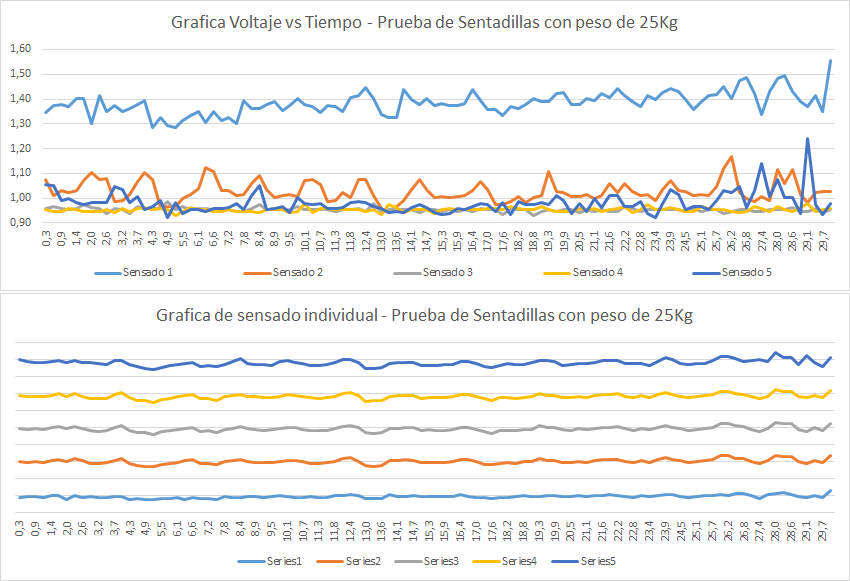
\includegraphics[width=1\textwidth]{./image/Grafica_Sentadillas.png}
%\caption{Gráfica de la prueba de sentadillas durante 30 segundos con pesas de 25Kg.}
%\label{fig:Grafica_Sentadillas}
%\end{figure}

\begin{figure}[H]
\centering
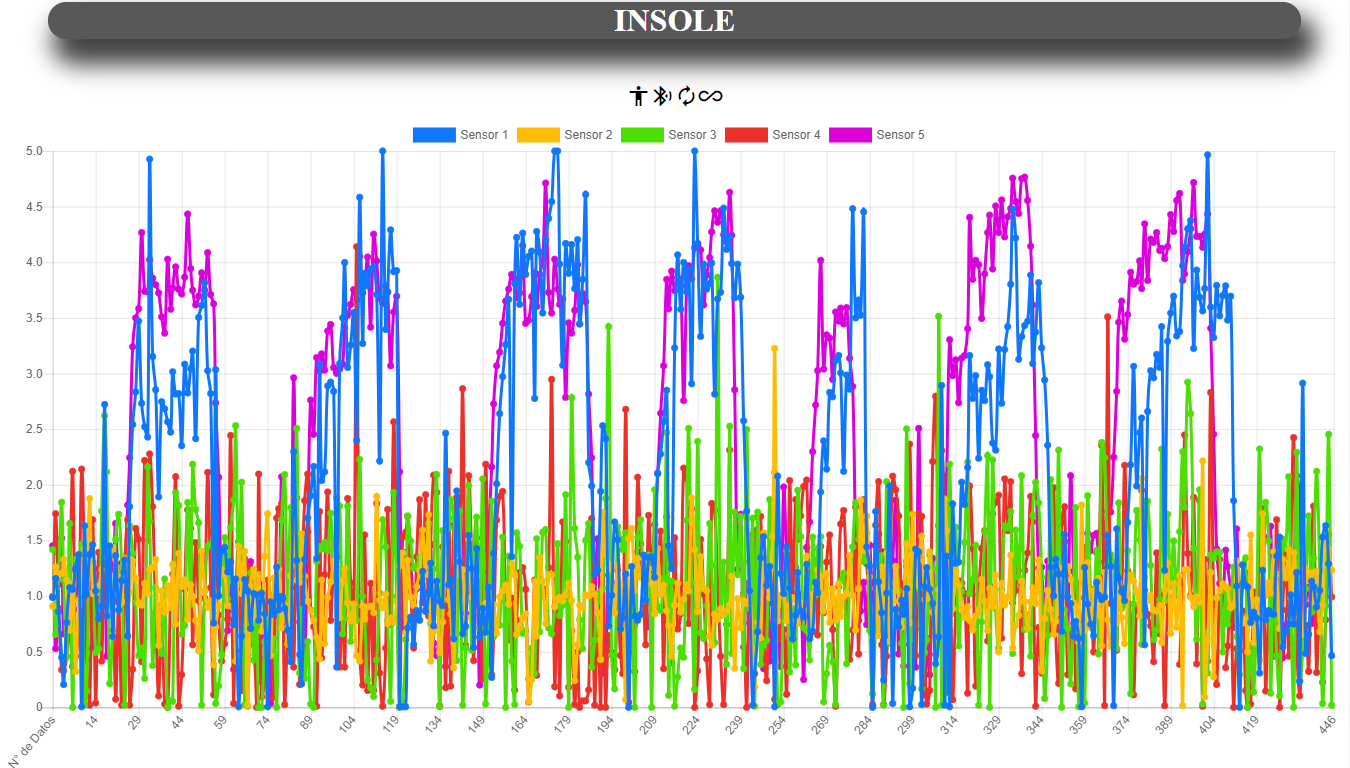
\includegraphics[width=1\textwidth]{./image/Insoleapp.png}
\caption{Gráfica de la prueba de Saltos durante 30 segundos.}
\label{fig:Grafica_Saltos}
\end{figure}

\begin{wrapfigure}{r}{0.2\linewidth}
\centering

\includegraphics[width=0.15\textwidth]{./image/Plantilla_Derecha.png}
\caption{Plantilla derecha con la ubicación de cada sensor.}
\label{fig:Plantilla_derecha}
\end{wrapfigure}

Se llevaron acabo pruebas para evaluar la comodidad y usabilidad del sistema, estas pruebas fueron usar la plantilla por debajo y por encima de la plantilla del calzado concluyendo así que para mayor comodidad del sistema, la plantilla diseñada debe ser usada por debajo de la plantilla del calzado deportivo.

Los resultados de las pruebas son trazados en la figura \ref{fig:Grafica_Saltos} se pueden observar los 7 valores por encima del promedio en la gráfica obtenida de la prueba de saltos \ref{fig:Saltos} observando los 7 saltos que fueron realizados en la prueba, se notan variaciones en el sensor numero 1 el cual esta ubicado en el dedo grueso y el sensor 5 ubicado en el talón.

El valor máximo de presión se registra en el centro del talón y el dedo grueso, en la practica de saltos primero se toma impulso sobre cargando la parte superior del pie para el salto y al final del movimiento sobre cargando la parte central del talón que es donde descansa la mayor parte del peso del cuerpo.

%\begin{figure}[H]
%\centering
%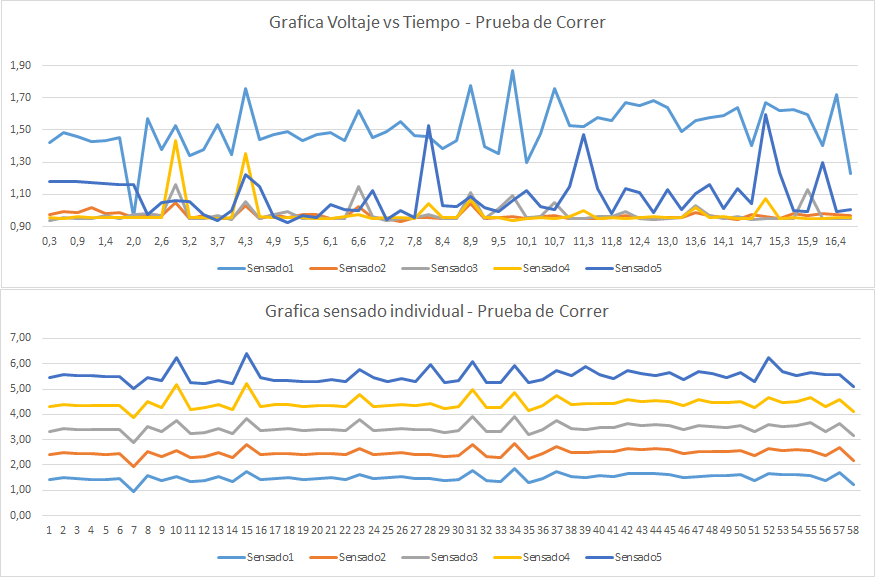
\includegraphics[width=1\textwidth]{./image/Grafica_Correr.png}
%\caption{Gráfica de la prueba de correr.}
%\label{fig:Grafica_Correr}
%\end{figure}



